\documentclass[twoside]{oss-conf-eng}
    % for slovak or czech use \documentclass[twoside]{oss-conf}
\usepackage[english,slovak]{babel}
    % use english and your language respectively ... czech, polish, ...
\usepackage[T1]{fontenc}
\usepackage[utf8]{inputenc}
\usepackage{amsmath}
\usepackage{amscd,amssymb,amsfonts}
\usepackage[sort,nocompress]{cite}
\usepackage{graphicx}                          % use for include pictures *.jpg, *.png, *.pdf
  %\usepackage{color}
  %\usepackage{colortbl}
  %\usepackage{multicol}
  %\usepackage{comment}
\usepackage{fancyhdr}
\usepackage[pdftex,unicode,bookmarks=false]{hyperref}  % for e-mail and url adress
\usepackage{listings}
\usepackage{eurosym}
\usepackage{lmodern}


%.............................................................................
\begin{document}
\def\keywordsnameS{Keywords}
%kohonen neural network, learning controll, iterative learning, PID controll, mobile robot}
%\def\keywordsnameS{Klíčová slova}    % pre češtinu odpoznámkovať

\setcounter{page}{1}                            % number of first page of article
\def\volumeDOI{OSSConf 2014:\  }                % proceedings information
\def\konfera{Konferencia OSSConf 2014}


\pagestyle{fancy}
\fancyfoot{}
\fancyhead[LE,RO]{\thepage}
\fancyhead[LO]{\nouppercase{\leftmark: \rightmark}}
\fancyhead[RE]{\nouppercase{\konfera}}


%.............................................. slovak or czech title
%          for shorts titles use command   \title{CELÝ NÁZOV ČLÁNKU}
\title[Klasifikácia žiadanej hodnoty Kohonenovou neurónovou sieťou]{Klasifikácia žiadanej hodnoty Kohonenovou neurónovou sieťou}


%.............................................. english title
%          for shorts titles use command   \titleA{THE TITLE OF ARTICLE}
\titleA[Required value classification using Kohonen neural network]{Required value classification using Kohonen neural network}


%............................. authors (first, second, ...) .. use next commands:
%
% \author[shorts]{Name Surname}{Title}{Past Title}{Country code}
% \address{address}
% \curraddress{current address}    alternative address
% \emailh{sanonymous@water.sun.xy}
% \urladdressh{http://www.sanous.tows.xy/~sanonymous}


\author[M. Chovanec]{Michal Chovanec}{Ing.}{}{}
\address{Department of Technical Cybernetics, Faculty of Management Science and Informatics,
University of Žilina, Univerzitná~8215/1, 010~26~Žilina, Slovak Republic}
% \curraddress{SOIT, 010~01 Žilina, Slovak Republic}
\emailh{michal.chovanec@yandex.com}
\urladdressh{http://aikenshin.blogspot.sk}

%.............................................. dedicatory
% \dedicatory{Dedicated to my hound\dots, optional}


%.............................................. keywords slovak/english
\keywords{kohonenová neurónová sieť, inteligentné učenie, iteraivne učenie, PID riadenie, mobilný robot}
\keywordsA{kohonen neural network, learning controll, iterative learning, PID controll, mobile robot}

%.............................................. (obligatory) AMS Classification 2000
% The 1-st classification is obligatory, the 2-nd classification is optional
% \subjclass{primary}{secondary}      f.e. \subjclass{35R35, 49N50}{}
  % \subjclass{35R35, 49M15, 49N50}{}



%.............................................. slovak Abstract
\selectlanguage{slovak}

\begin{abstract}
V článku je popísaná klasifikácia situacií Kohonenovou neurónovou sieťou.
Výsledky sú demonštrované na robotovi, sledujúom čiaru, kde sú klasifikované rôzne
typy zákrut. Každá situácia má zodpovedajúci výstup, ktorý je vstupom do nižšej úrovne riadenia.
\end{abstract}


%.............................................. english Abstract
\selectlanguage{english}

\begin{abstractA}
In this paper we describe situations classification using Kohonen neural network.
Results are demonstrated on line following robot, where different curves are classified.
Each classificated situation has corresponding required value output,
which is used by low level control process.
Network weights estimates are processed in real time.
\end{abstractA}



\selectlanguage{english}
%........................... private macros (f.e. the different environments)
\newtheorem{theorem}{Theorem}[section]
\newtheorem{corollary}[theorem]{Corollary}
\newtheorem{lemma}[theorem]{Lemma}
\newtheorem{exmple}[theorem]{Example}
\newtheorem{defn}[theorem]{Definition}
\newtheorem{proposition}[theorem]{Proposition}
\newtheorem{conjecture}[theorem]{Conjecture}
\newtheorem{rmrk}[theorem]{Remark}
            %%% for no-italic, numbered environments, use:
\newenvironment{definition}{\begin{defn}\normalfont}{\end{defn}}
\newenvironment{remark}{\begin{rmrk}\normalfont}{\end{rmrk}}
\newenvironment{example}{\begin{exmple}\normalfont}{\end{exmple}}
            %%% for unnumbered environments, use f.e.
\newtheorem*{remarque}{Remark}
\newcommand\bbreak{\allowdisplaybreaks}
\newcommand\dd{\mathop{\rm d\!}\nolimits}
\newcommand\sgn{\mathop{\rm sgn}\nolimits}


%.............................................. maketitle
\maketitle

%.............................................. the main article

\section*{Introduction}

It is well known that, iterative learning control can handle any repetitive control
process \cite{ilc1}, \cite{ilc2}. Most of applications we can found in manipulators
control in industry.

Some problems have iterative (or semiterative) character, but more than one
output sequence is required. Consider problem of line following robot. To control robot
speed, it is necessary to know curve shape. If we can compute associative memory, where input is
line shape and output is required speed, we can handle this problem.

\section{Problem formalisation}

Consider two wheels (two motors) robot with differential drive \cite{robot_model_1}. For motors
control signals we can write

\begin{eqnarray}
\begin{split}
\label{robot_equation}
	r(n) &=	v(n) - d(n), \\
    l(n) &=	v(n) + d(n),
\end{split}
\end{eqnarray}

where \\
$r(n)$ ($l(n)$) is right (left) motor control output,
$v(n)$ is common control input,
$d(n)$ is difference control input.
\\
The value of $d(n)$ can be computed with sufficient precision using PD controller \cite{servo_pd}. Our goal
is to properly estimate $d(n)$ which is speed of robot.
Robot motion equations can be written as
\begin{eqnarray}
\begin{split}
\label{robot_equation}
	\theta(n) &= (1 + \alpha) \theta(n-1) - \alpha \theta(n-2) + b_0 (r(n) - l(n))  \\
    \nu(n) &=  \alpha \nu(n-1) + (1 - \alpha) b_1 (r(n) + l(n))
\end{split}
\end{eqnarray}

where \\
$\theta$ is robot orientation (Yaw angle),
$\nu$ is robot speed,
$\alpha$ is robot inertia constant, within $(0, 1)$,
$b_0$ and $b_1$ are constants dependent on wheel distances, wheel diameters, gear ratio, and
maximum speed.

If required $\theta$ and $\nu$ are known, we can successfully use pure PID control defining error
as $e_{\theta}(n) = \theta_r(n) - \theta(n)$, $e_{\nu}(n) = \nu_r(n) - \nu(n)$, where $\theta_r(n)$
and $\nu_r(n)$ are required values.
In our line following problem, $\nu_r(n)$ is unknown, value $\theta(n)$ is readed from
line position sensor. In fact, inertia of motors is much
smaller than inertia of whole robot, for control $\theta(n)$ we can still use PD
controller. Let the required value be $\theta_r(n) = 0$, which means robot is straight on line.

Our goal is to properly estimate $v(n)$ and control robot speed, to give enough time
for PD control to setup $\theta(n)$. We are minimizing $e_{\theta}(n)$ and maximizing $\nu(n)$
(corespoding to $v(n)$).


%%%%%%%%%%%%%%%%%%%%%%%%%%%%%%%%%%%%%%%%%%%%%%%%%%%%%%%%%%%%%%%%%%%%%%%%%%%%%%
\section{Controller design}

On figure \ref{fig:robot_controller} we can sse block diagram of proposed controller.

\begin{figure}[]
    \centering
    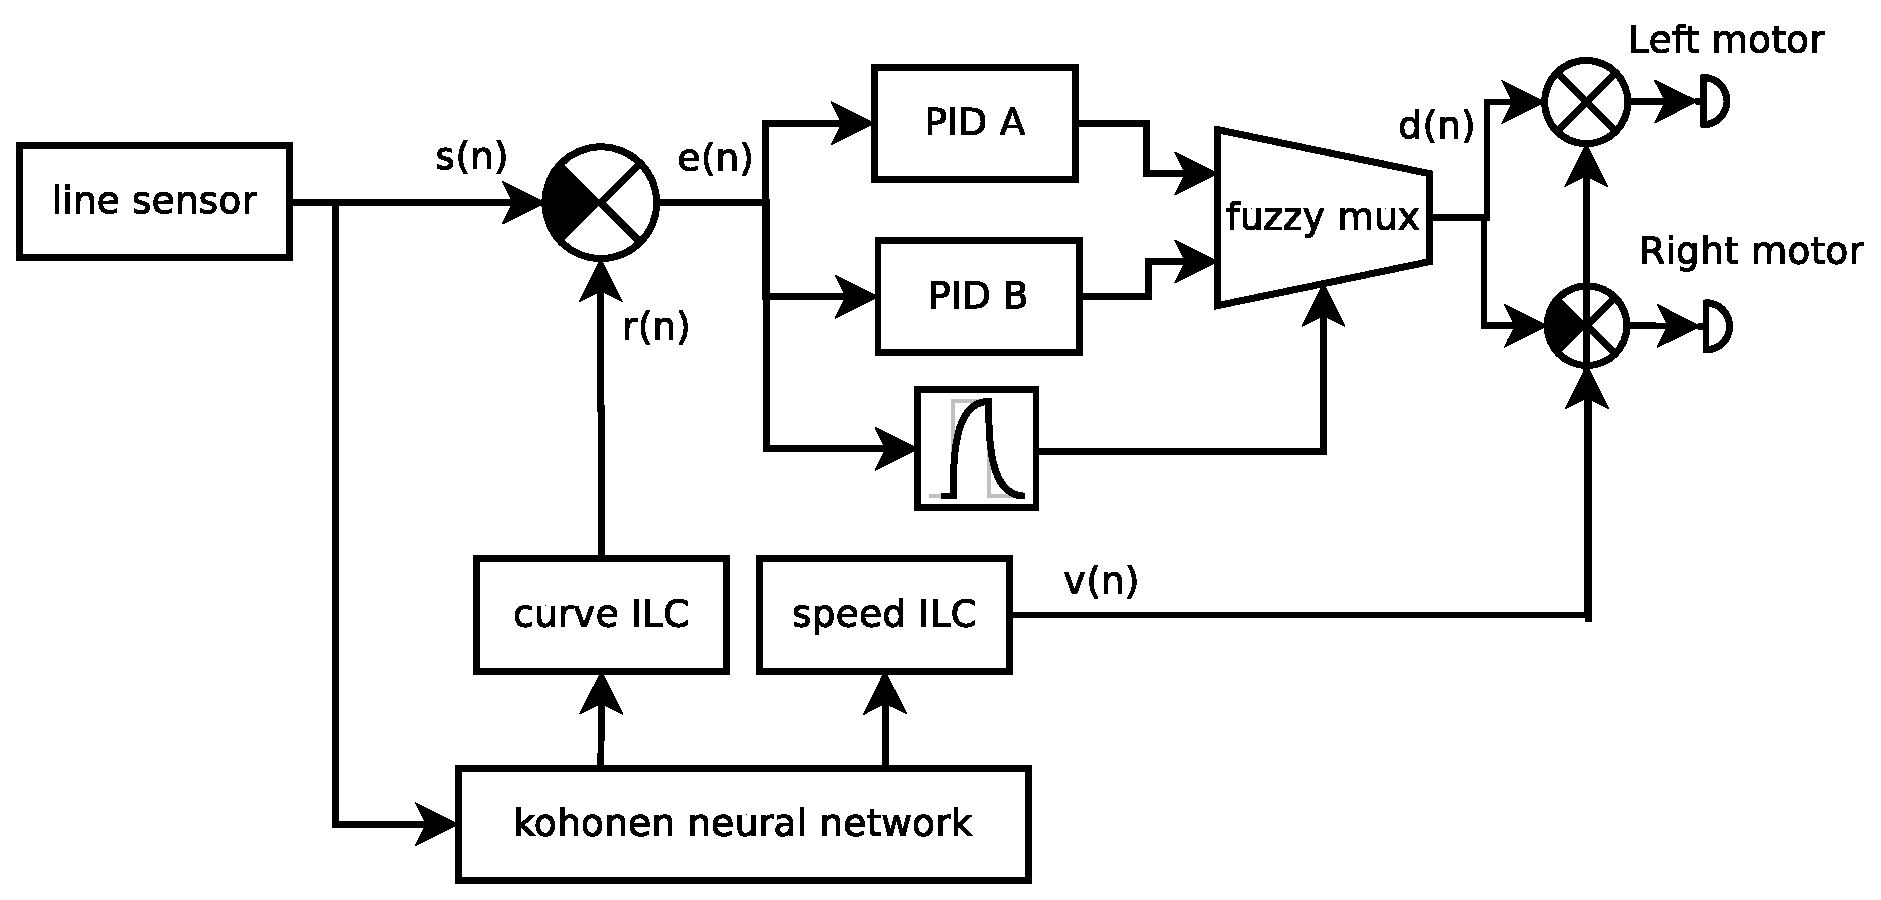
\includegraphics[width=0.8\textwidth]{block_diagram/robot_block.eps}
    \caption{Robot controller}
    \label{fig:robot_controller}
\end{figure}

Input is line position from sensor $s(n)$. All values are normalised into
$\langle -1, 1 \rangle$.
Required value of $\theta(n)$ is marked as
$r(n)$. In simplificated case, it can be set to 0. Computed error is used as input into two
PD controllers (PID in general, I-term is equal to zero, because \ref{robot_equation}
($\theta$ part) has pole on $1 + 0i$. If I-term is nonzero, there will be secondorder pole on $1 + 0i$ and
system will be unstable).

PD controller outputs are mixed using fuzzy mux, which works as

\begin{eqnarray}
\begin{split}
\label{fuzzy_mux}
	d(n) &= s'(n)a(n) + (1 - s'(n))b(n)
\end{split}
\end{eqnarray}

where \\
$a(n)$ is PID A output,
$b(n)$ is PID B output,
$s'(n)$ is select input, from interval $\langle 0, 1 \rangle$. \\

Select output is produced by nonlinear low pass filtered signal of $e(n)$ as

\begin{eqnarray}
\begin{split}
\label{low_pass}
s'(n) =
  \begin{cases}
    s'(n-1)k + (1 - k)|e(n)| & \text{for} |e(n)| < s'(n-1), \\
    |e(n)| & otherwise,
  \end{cases}
\end{split}
\end{eqnarray}

where $k$ is filter constant, from $(0, 1)$. This filter is smoothing error
values.

This system properly switches between two controllers, one for straight line and
one for curved line.

To estimate $v(n)$ we use Kohonen neural network \cite{kohonen_neural_network}
 and iterative learning control. Neural network input is vector of $s(n)$ values
(implemented as FIFO, in experiments with size M = 16). Mark this vector as $S(n) =
[s(n), ..., s(n - M)]$.

Our goal, is to train network to make the classification of vectors $S(n)$. Depending on count of classification classes,
we choose corresponding neurons count $N$. In experiments chooses we take $N=16$ which means, 16 different
curve shapes can be recognized.

Transfer function of j-th neuron can be written as

\begin{eqnarray}
\begin{split}
\label{neuron_transfer}
y_j(n) = \sum_{i = 0}^{M-1} {|s(n-i) - w_j(i)|}
\end{split}
\end{eqnarray}

where $w_j$ are neuron weights, initially chosen randomly
 and modified during learning process.

Neuron with smaller $y_q(n)$ will be marked as winning neuron, and weights modification
will be done by formulae

\begin{eqnarray}
\begin{split}
\label{neuron_transfer}
w_q(n) = \eta w_q(n-1) + (1 - \eta)S(n),
\end{split}
\end{eqnarray}

where $\eta$ is learning rate, from $(0, 1)$ close to 1. Weights of neurons are slowly adapted
to corresponding pattern. This can be illustrated on figure \ref{fig:kohonen_test_01}. Input was
2 dimensional, and goal is to find centers (green) of some data set (red). Input
data set was produced by some Markov process. On figure \ref{fig:kohonen_test_02} $y_q(n)$ values are shown.

\begin{figure}[]
    \centering
    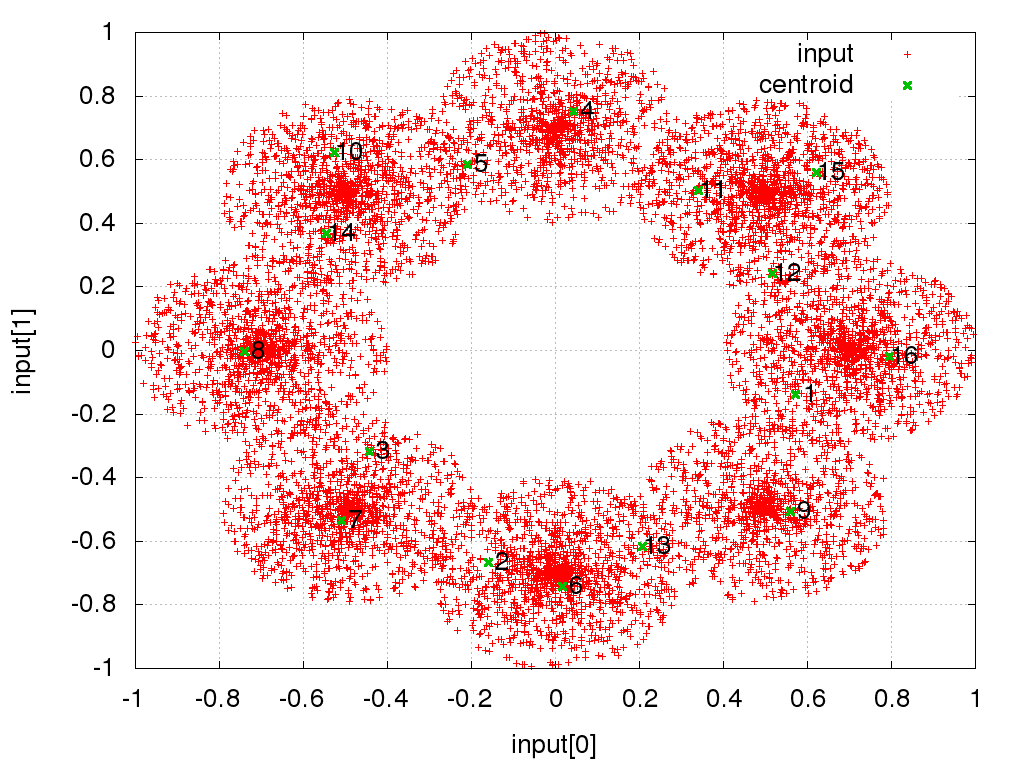
\includegraphics[width=0.6\textwidth]{kohonen_test/learing_result.png}
    \caption{Kohonen test}
    \label{fig:kohonen_test_01}
\end{figure}

\begin{figure}[]
    \centering
    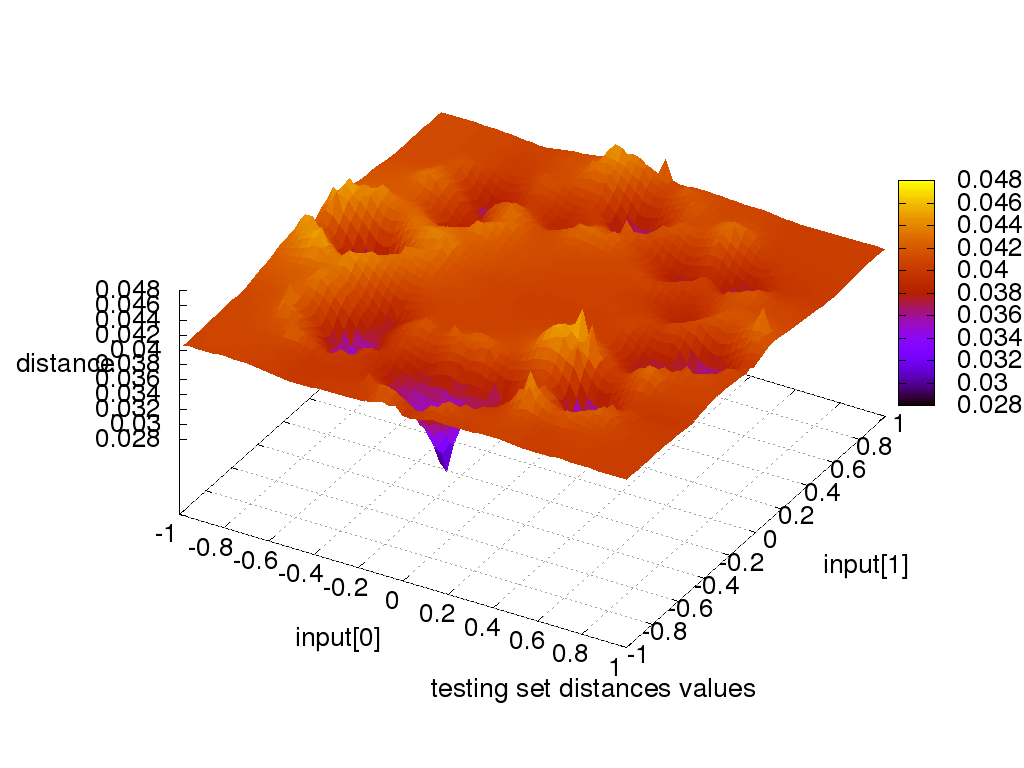
\includegraphics[width=0.7\textwidth]{kohonen_test/distances_result.png}
    \caption{Kohonen test distances}
    \label{fig:kohonen_test_02}
\end{figure}

After found winning neuron, we need to find corresponding $v(n)$, denote it by
$v_q(n)$.


\begin{eqnarray}
\begin{split}
\label{speed_estimating}
v_q(n) = v_q(n-1) + 1 - k\;s_f(n) ,
\end{split}
\end{eqnarray}

where $s_f(n)$ is low pass filtered $s(n)$ value.
That means robot speed $v(n)$ on curve type $q$ is rising if $s_f(n)$ is low.

\section{Experimental results}

Robot was learning for few loops on short line race with different curve types.
Resulting curve types are on figure \ref{fig:curves}. Each line represents
one curve shape. To reduce space in memory, absolute value of $s(n)$ as input into
Kohonen neural network is used. We can seen many straight line positions, and
few curves.

\begin{figure}[]
    \centering
    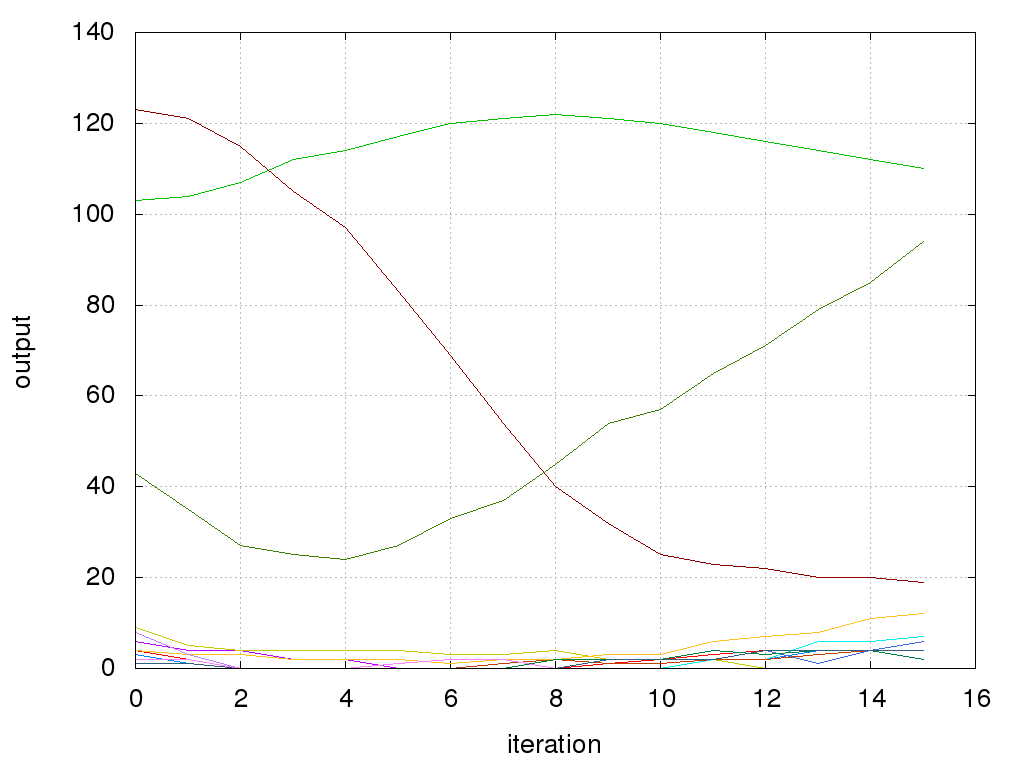
\includegraphics[width=0.6\textwidth]{prediction/predictor.png}
    \caption{Resulting curves types}
    \label{fig:curves}
\end{figure}

\section{Conclusions}

In paper  learning system for curve shape recognition using Kohonen
neural network was described. Neural network results have corresponding speed output which control
robot optional speed. Learning process is working in real time,
on 75MHz ARM Cortex M4F microcontroller. Robot is on figure \ref{fig:robot}.
Robot working video can be seen on \cite{robot_video}. More pictures are
available on authors blog \cite{blog} and sources on github \cite{git}.

\begin{figure}[]
    \centering
    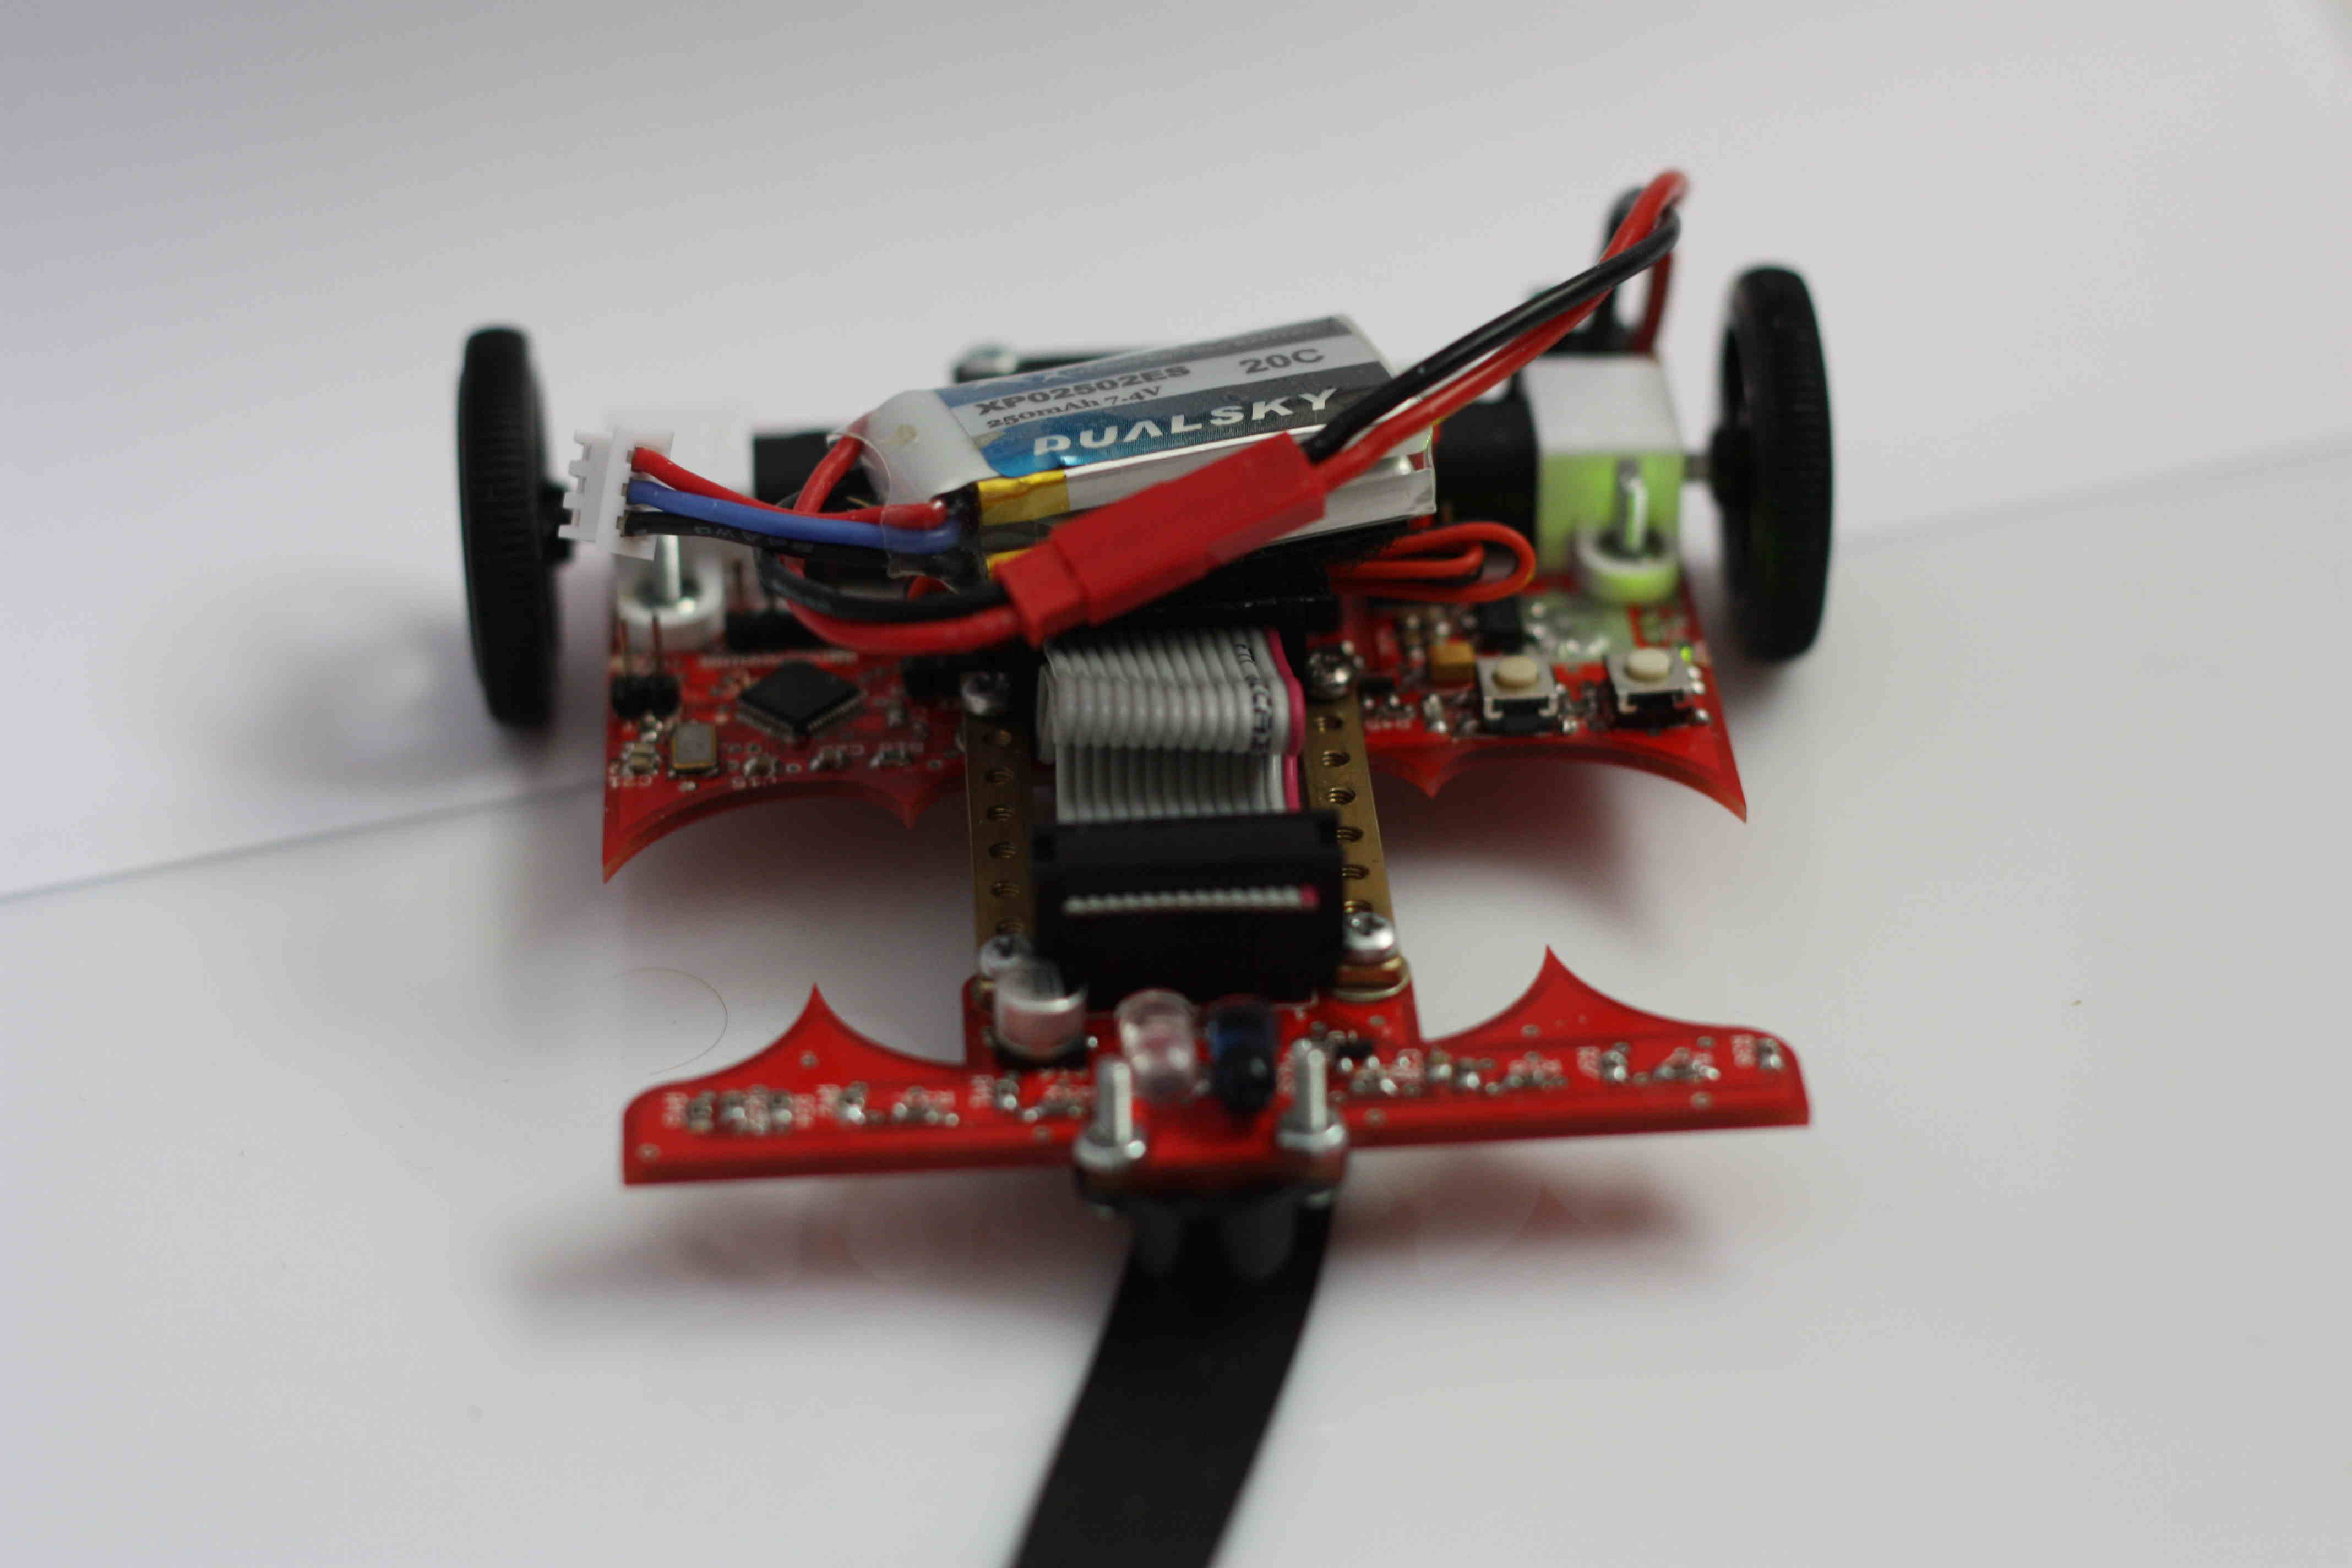
\includegraphics[width=0.5\textwidth]{motoko_aftermath_front.jpg}
    \caption{Testing robot}
    \label{fig:robot}
\end{figure}


%============================================================================%
%                                references                                  %
%============================================================================%
\begin{thebibliography}{99}

\bibitem{ilc1}
Kevin L. Moore: Iterative learning control
\url{http://inside.mines.edu/~kmoore/survey.pdf}.

\bibitem{ilc2}
Kevin L. Moore: An Introduction to Iterative Learning Control
\url{http://inside.mines.edu/~kmoore/ilc-intro-pdftex03-03.pdf}.

\bibitem{robot_model_1}
Patrícia N. Guerra: Linear modelling and idendification of a mobile robot with
differential drive
\url{http://www.dca.ufrn.br/~adelardo/artigos/ICINCO04b.pdf}.

\bibitem{kohonen_neural_network}
R. Rojas: Neural Networks, Springer-Verlag, Berlin, 1996, Kohonen Neural Networks
\url{http://page.mi.fu-berlin.de/rojas/neural/chapter/K15.pdf}

\bibitem{servo_pd}
Michael Goldfarb, Taweedej Sirithanapipat:
The effect of actuator saturation on the performance of PD-controlled servo systems
\url{http://research.vuse.vanderbilt.edu/cim/pubs/journal/35%20-%20Goldfarb%20and%20Sirithanapipat.pdf}.

\bibitem{robot_video}
robot video link
\url{https://www.youtube.com/watch?v=SGaNlbkyQMg}.

\bibitem{blog}
authors blog
\url{http://aikenshin.blogspot.sk/}.

\bibitem{git}
authors github
\url{https://github.com/michalnand/motoko_after_math_linefollower}.

\end{thebibliography}

\end{document}
%%%%%%%%%%%%%%%%%%%%%%%%%%%%%%%%%%%%%%%%%%%%%%%%%%%%%%%%%%%%%%%%%%


%
